\documentclass[a4paper, 12pt]{article}
\usepackage[left=2cm,right=2cm,top=2cm,bottom=2cm]{geometry}
\setlength{\parindent}{0cm}
\usepackage{graphicx}
\usepackage{kvsetkeys}
\begin{document}

\title{Assignment-4 (MM2090)}
\author{Arun Palaniappan}
\date{28 june 2021}
\maketitle

\section{Arun Palaniappan ME20B036}

General Time-delay with single-fractional-pole model (TDSFP)~\cite{YUAN2022108111} :

\begin{equation}
 \mathcal{L}^{-1}\left \{\frac{s^{\alpha-\beta}}{s^{\alpha} + a} \right\} = t^{\beta-1}E_{\alpha,\beta}(-at^{\alpha})
 \label{eqn:equation}
\end{equation}

\subsection{Analysis}
Following contains a brief explanation of the variables and the importance of the equation :
\begin{itemize}

    \item From equation~\ref{eqn:equation}, `$\mathcal{L}^{-1}$' is the inverse Laplacian operator, which plays a major role in deducing the solution.
    \item From equation~\ref{eqn:equation}, `$E_{\alpha,\beta}$' is the Mittag-Leffler function
    \item `$\alpha,\beta$' are the parameters of the Mittag-Leffler function
    \item From equation~\ref{eqn:equation}, `s' is the parameter of the TDSFP transfer function
    \item `a' defines the system order during the process
    \item `t' denotes the time from the start of the process
\end{itemize}
Modeling of the ideal thermal conduction process is a classical application of TDSFP model. Physically the heat equation describes how temperature evolves over time in a solid medium. It describes the distribution in only one spatial coordinate, and the heat transferred in the direction in which the temperature decreases.~\cite{YUAN2022108111}

\begin{figure}[h]
	\begin{center}
		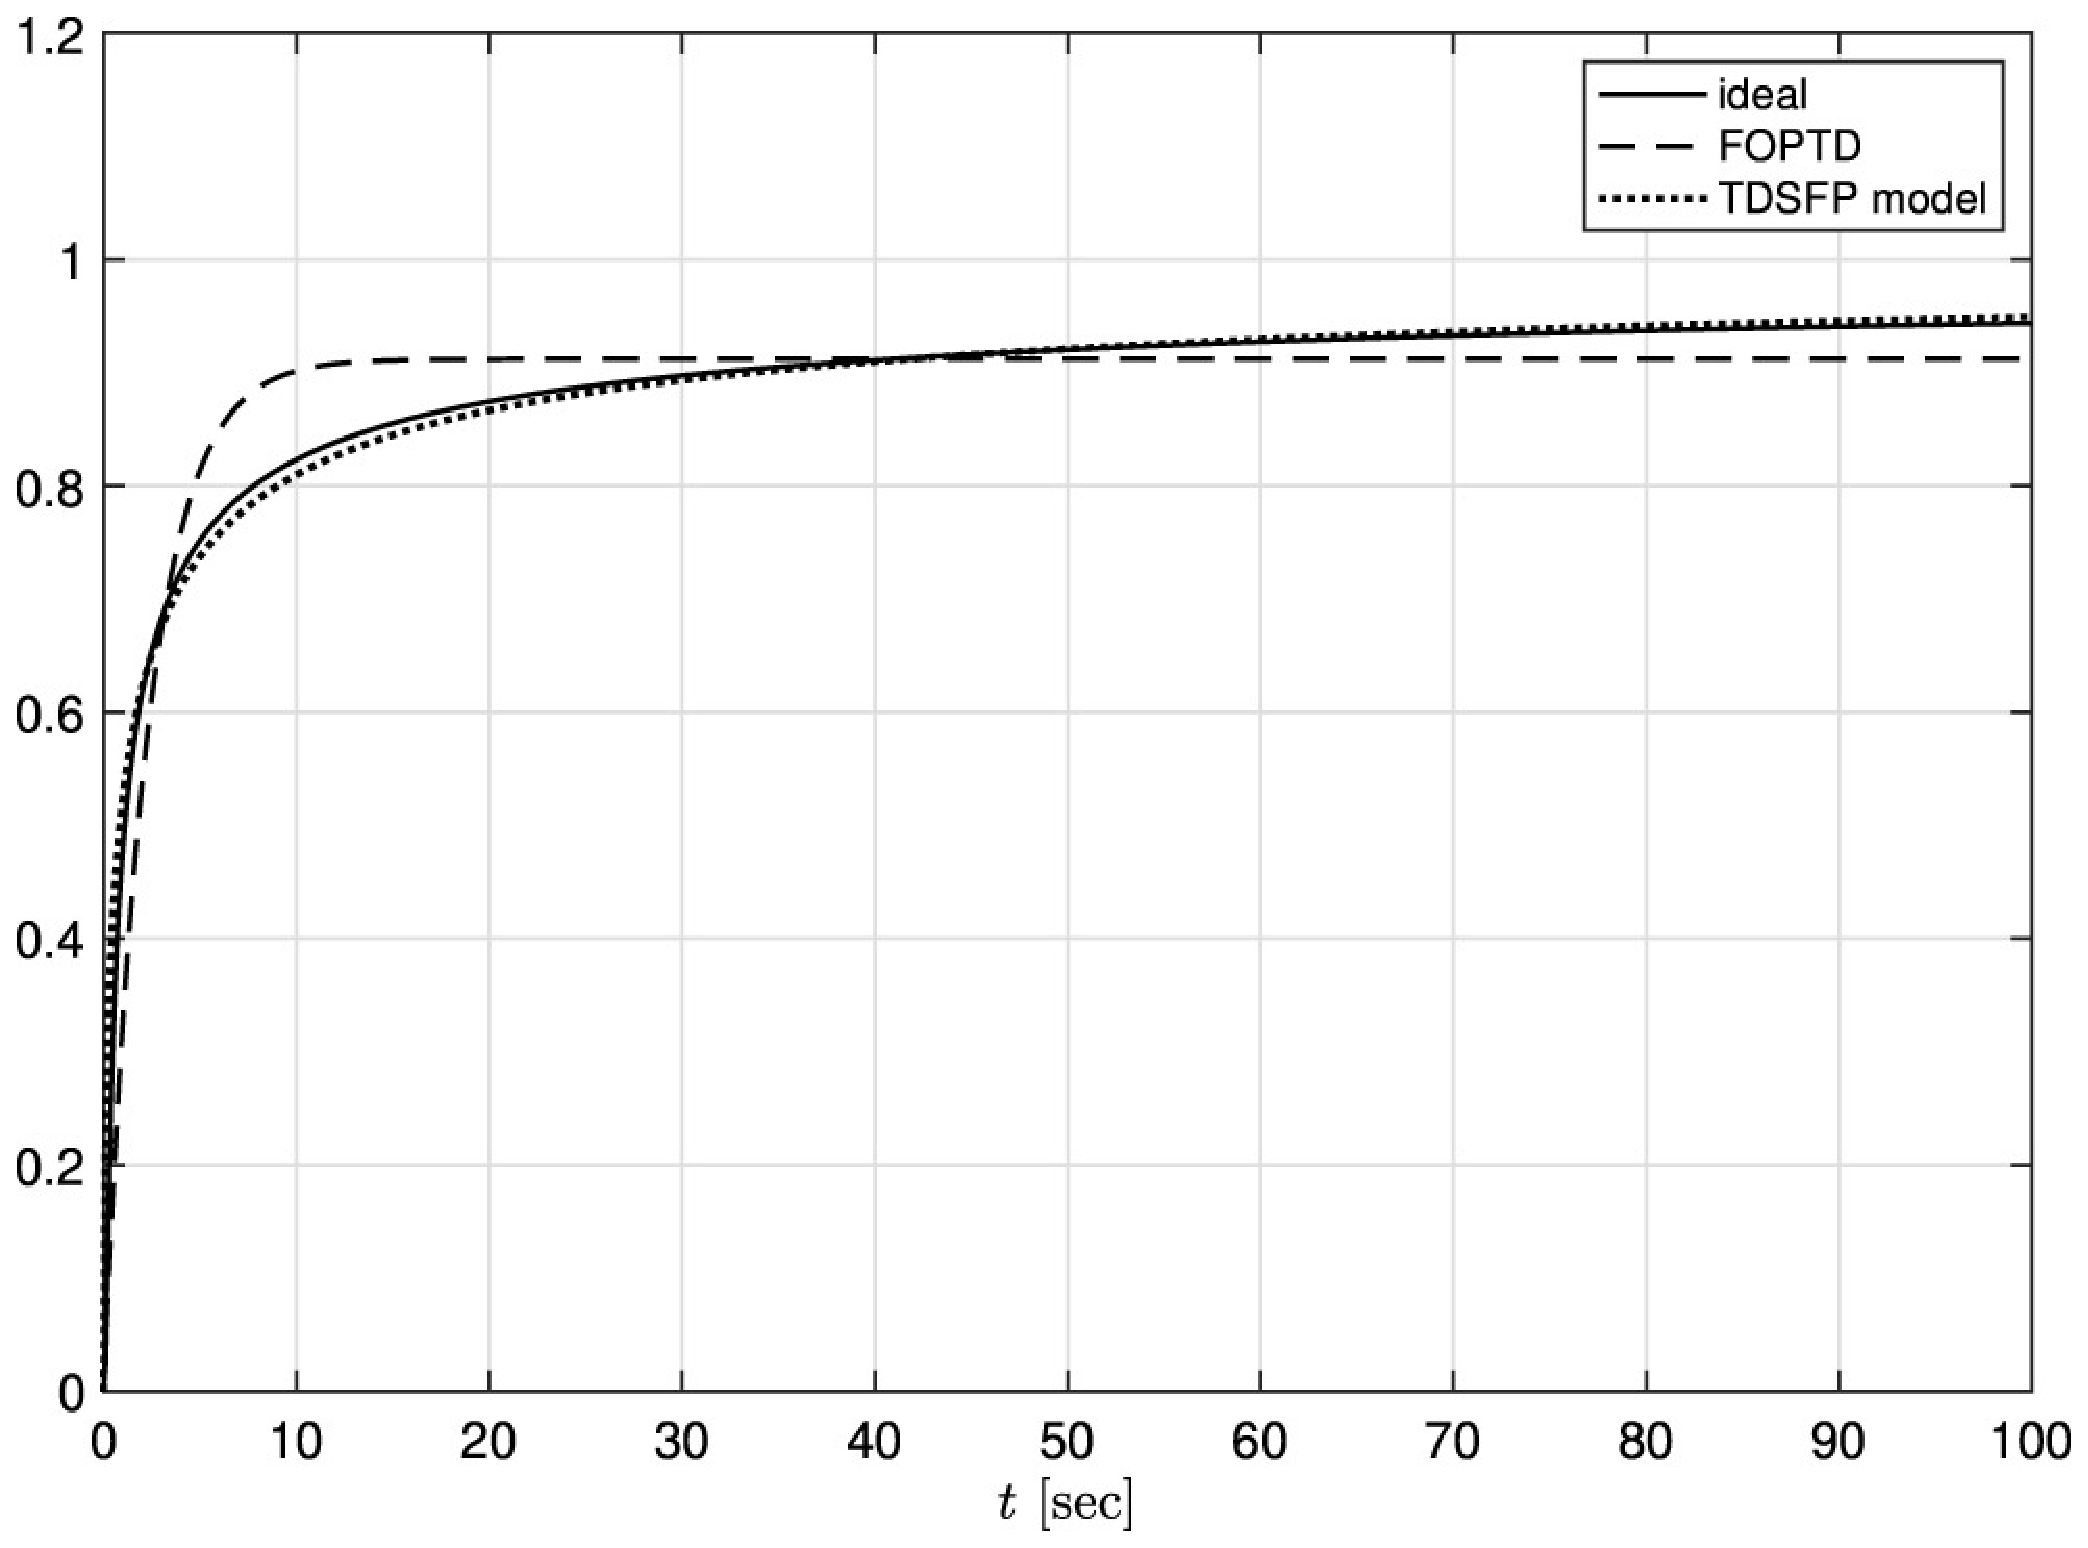
\includegraphics[scale=0.3]{Assgt4.eps}
	\end{center}
	\caption{ME20B036}
	\label{f1:image}
\end{figure}


Figure~\ref{f1:image} shows the graph plot of the TDSFP model.~\cite{YUAN2022108111}

%\bibliography{Team-1.bib}
%\bibliographystyle{plain}

\end{document}
